\documentclass[11pt,a4paper]{article}
\usepackage[utf8]{inputenc}
\usepackage[T1]{fontenc}
\usepackage[brazil]{babel}
\usepackage[dvipsnames]{xcolor}
\usepackage{amsmath,amsthm,bm,mathtools}
\usepackage{newtxtext,newtxmath}
\usepackage[margin=2.25cm,top=2.25cm,bottom=2.25cm]{geometry}
\usepackage{microtype,booktabs,tabularx,array,graphicx,float}
\usepackage{enumitem}
\usepackage{fancyhdr}
\usepackage{hyperref}
\usepackage{cleveref}
\hypersetup{colorlinks=true,linkcolor=MidnightBlue,citecolor=MidnightBlue,urlcolor=MidnightBlue,
 pdftitle={Q-Learning contínuo e aprendizagem ortogonal de respostas relativas para desfechos binários},
 pdfauthor={Manuscrito metodológico de trabalho},pdfsubject={Tratamento contínuo, risk ratio, elasticidade e double machine learning}}
\setlength{\parskip}{0.32em}
\setlength{\parindent}{1em}
\setlength{\headheight}{15pt}
\pagestyle{fancy}
\fancyhf{}
\fancyhead[L]{\small Q-Learning contínuo e respostas relativas}
\fancyhead[R]{\small Manuscrito de trabalho}
\fancyfoot[C]{\small\thepage}
\renewcommand{\headrulewidth}{0.25pt}
\setlist{nosep,leftmargin=*}
\newtheorem{theorem}{Proposição}[section]
\newtheorem{corollary}[theorem]{Corolário}
\newtheorem{remark}[theorem]{Observação}
\newcommand{\E}{\mathbb E}
\newcommand{\Pp}{\mathbb P}
\newcommand{\R}{\mathbb R}
\newcommand{\ind}{\mathbf 1}
\newcommand{\Var}{\operatorname{Var}}
\newcommand{\Cov}{\operatorname{Cov}}
\newcommand{\logit}{\operatorname{logit}}
\newcommand{\KL}{\operatorname{KL}}
\newcommand{\op}{o_{\Pp}}
\newcommand{\Op}{O_{\Pp}}
\DeclareMathOperator*{\argmin}{arg\,min}
\title{\vspace{-0.9cm}\textbf{Q-Learning contínuo e aprendizagem ortogonal\newline de respostas relativas para desfechos binários}\\[0.4em]
\large Identificação por densidades, momentos multiplicativos\newline e validação por intervenções estocásticas}
\author{Manuscrito metodológico de trabalho}
\date{5 de setembro de 2026}
\begin{document}
\maketitle
\thispagestyle{empty}
\begin{abstract}
Em problemas de precificação com conversão binária, efeitos causais em pontos percentuais podem ordenar indivíduos quase exclusivamente pela conversão-base, mesmo quando a resposta proporcional ao preço é constante. Desenvolvemos uma extensão contínua da perspectiva Q-Learner, distinguindo três objetos: a identidade não paramétrica que expressa razões de conversão como razões de densidades de tratamento; um estimador ortogonal de curvas multiplicativas com forma especificada; e um estimador de razões entre respostas a intervenções estocásticas fixas, sem impor uma curva log-linear. A identidade de Bayes produz diretamente a log-resposta relativa e sua derivada. Para o modelo multiplicativo, apresentamos um momento de G-estimação com viés condicional exatamente igual a um produto de erros e estabelecemos condições suficientes de inferência com cross-fitting para um parâmetro de dimensão fixa. Para a construção não paramétrica, derivamos sinais aumentados e uma equação de estimação de razões que preserva dupla robustez de consistência, evitando dividir pseudo-outcomes individuais. Expomos as limitações de suporte, regularidade, compatibilidade probabilística e inferência sob misspecificação. Em 100 replicações sintéticas de 30 mil observações, com conversão esperada de 6\%, os testes reproduzem a robustez do momento multiplicativo e a vulnerabilidade do Q-Learner simples à densidade incorreta. Uma realização adicional com 100 mil observações e nuisances estimadas por boosting ilustra o algoritmo com cross-fitting. Um pacote Python acrescenta APIs discretas e contínuas; dez novos cenários com 30 replicações, 12 mil registros de treino e 2 mil de teste independente por cenário avaliam lift, curvatura, conversão rara e estabilidade, após uma rodada piloto preservada. O manuscrito conecta resultados existentes; não reivindica prioridade sobre Bayes, G-estimação, DML ou modelos multiplicativos contínuos, nem apresenta validação em dados reais.
\end{abstract}
\noindent\textbf{Palavras-chave:} tratamento contínuo; outcome binário; risco relativo; elasticidade; generalized propensity score; orthogonal machine learning; financiamento de veículos.

\section{Motivação, escopo e relação com a literatura}
\label{sec:intro}
Considere clientes que simularam um financiamento e foram aprovados por crédito. A resposta observada é a contratação dentro de uma janela previamente definida. Em um funil cuja conversão média é aproximadamente 6\%, há segmentos que convertem muito menos e outros que convertem perto de 25\%. Uma mudança de taxa que aumenta a conversão proporcionalmente em 20\% produz ganhos absolutos de 0,4 ponto percentual quando a conversão-base é 2\%, mas de 5 pontos percentuais quando a conversão-base é 25\%. Não há contradição: heterogeneidade absoluta e heterogeneidade relativa são alvos diferentes.

Para duas doses $t$ e $t_0$, escreva $\mu(t,x)=\Pp\{Y(t)=1\mid X=x\}$. A decomposição
\begin{equation}
\mu(t,x)-\mu(t_0,x)
=\mu(t_0,x)\left\{\frac{\mu(t,x)}{\mu(t_0,x)}-1\right\}
\label{eq:decomp}
\end{equation}
mostra que um CATE aditivo pode reproduzir o ranking de conversão-base sem existir heterogeneidade relativa. A ortogonalização usada em DML não elimina uma associação causal verdadeira entre efeito absoluto e baseline. Nosso objetivo é representar explicitamente a \emph{forma relativa da curva de conversão}, mantendo sua escala absoluta disponível para avaliar valor econômico.

\subsection{O que o artigo motivador faz e o que não faz}
\emph{Beyond Differences}, de Fuchs e Kreiss \cite{fuchs2026}, formula o problema com tratamento e outcome binários. Sua Observação 2 apresenta uma extensão da identidade Q-Learner a múltiplas classes. A v1 consultada não desenvolve uma teoria para densidades contínuas, derivadas de dose-resposta ou inferência contínua. Substituir probabilidades de braços por densidades é uma extensão algébrica natural; não basta, porém, para obter dupla robustez ou intervalos de confiança válidos.

Também seria incorreto dizer que efeitos multiplicativos com tratamento contínuo e outcome binário são novos. Yin et al. \cite{yin2022} estudam precisamente esse domínio e discutem compatibilidade de probabilidades, parametrizações e G-estimação. Dukes e Vansteelandt \cite{dukes2018} apresentam G-estimação de riscos relativos; Yadlowsky et al. \cite{yadlowsky2021} tratam estimação e validação de CATEs por razão. As construções de DML e de resposta causal contínua estão estabelecidas em Chernozhukov et al. \cite{chernozhukov2018}, Kennedy et al. \cite{kennedy2017} e Colangelo e Lee \cite{colangelo2020}. Ge e Díaz \cite{ge2026} desenvolvem aprendizagem ortogonal de razões para tratamento binário. Shinoda e Hoshino \cite{shinoda2022} estudam razões de funções de esperança condicional.

\subsection{Contribuição e status deste manuscrito}
O desenvolvimento a seguir organiza uma ponte entre essas perspectivas: a identidade Q contínua separa nível e forma; a G-estimação multiplicativa fornece um momento simples sem estimar a densidade inteira; intervenções suavizadas fornecem alvos não paramétricos com sinais aumentados exatos. A denominação \textbf{CQ-DML} é apenas um nome de trabalho para essa implementação ortogonal, e não uma alegação de invenção da G-estimação.

As proposições são acompanhadas de demonstrações e os resultados numéricos foram efetivamente executados em dados sintéticos. Não houve acesso à base de financiamento, revisão por pares ou verificação bibliográfica exaustiva de prioridade. As taxas assintóticas são afirmadas apenas para os alvos e regimes explicitamente especificados. Em particular, não se reivindica inferência $\sqrt n$ para uma superfície condicional arbitrária em alta dimensão.

\section{Definições e identificação causal}
\label{sec:setup}
Observamos $O=(X,T,Y)$, com $Y\in\{0,1\}$ e dose $T\in\mathcal T_x\subseteq\R$. Usamos $T$ para a variável de tratamento/taxa, $t$ para seu valor e $t_0$ para a referência. As covariáveis $X$ são anteriores à intervenção. Inicialmente, consideramos observações independentes; para simulações repetidas do mesmo cliente, o particionamento e a inferência devem respeitar os clusters.

Assumimos consistência $Y=Y(T)$, ausência de interferência relevante e intercambialidade condicional $Y(t)\perp T\mid X$ para as doses de interesse. Sob essas hipóteses,
\[
\mu(t,x)=\E[Y\mid T=t,X=x].
\]
Para tratamentos contínuos, igualdades condicionais valem quase em toda parte; a identificação em pontos determinados requer uma versão regular, por exemplo contínua em $t$. A interpretação causal depende dessas hipóteses; a identidade de Bayes apresentada adiante, por si só, é apenas probabilística.

Denote por
\begin{align}
f(t\mid x)&=f_{T\mid X}(t\mid x),&
p(x)&=\Pp(Y=1\mid X=x)=\int\mu(u,x)f(u\mid x)\,du,\label{eq:defs}\\
q(t\mid x)&=f_{T\mid X,Y=1}(t\mid x).&&\notag
\end{align}
Aqui $f$ é a densidade de alocação do tratamento; $p$ é a conversão sob a política observada; e $q$ é a densidade da dose entre conversores. Em geral, $p(x)\ne\mu(t_0,x)$.

Escolha uma referência pré-especificada $t_0(x)$ no suporte de interesse. Os alvos são
\begin{align}
R(t,t_0;x)&=\frac{\mu(t,x)}{\mu(t_0,x)},&
g(t,t_0;x)&=\log R(t,t_0;x),\label{eq:targets}\\
s(t,x)&=\partial_t\log\mu(t,x).&&\notag
\end{align}
São necessárias conversões de referência estritamente positivas. Quando $T=r$ é a taxa bruta positiva, a elasticidade é $\varepsilon(r,x)=r\,s(r,x)$. Quando $T=\log\{r/r_{\mathrm{base}}(x)\}$, com taxa-base pré-tratamento, $s(t,x)$ já é a elasticidade em relação a $r$. Uma normalização adicional $T=\log\{r/r_{\mathrm{base}}(x)\}/c$ implica $\varepsilon=s/c$.

\begin{remark}[Unidades e população]
Uma alteração de 0,1 ponto percentual na taxa mensal não equivale a uma alteração relativa de 10\%. O estimando deve fixar a convenção. O recorte de clientes aprovados é admissível como população-alvo se aprovação e entrada no funil antecedem a intervenção. Se a taxa testada altera a probabilidade de entrar no recorte, há seleção pós-tratamento, que não é corrigida pela escolha da escala relativa.
\end{remark}

\section{A extensão contínua do Q-Learner}
\label{sec:q}
\begin{theorem}[Identidade Q contínua]
\label{prop:bayes}
Se $p(x)>0$ e $f(t\mid x)>0$ no domínio avaliado, então
\begin{equation}
q(t\mid x)=\frac{\mu(t,x)f(t\mid x)}{p(x)}.
\label{eq:bayes}
\end{equation}
Consequentemente, quando $\mu(t_0,x)>0$,
\begin{equation}
\boxed{R(t,t_0;x)=\frac{q(t\mid x)}{q(t_0\mid x)}
                           \frac{f(t_0\mid x)}{f(t\mid x)}.}
\label{eq:qratio}
\end{equation}
Se as funções são diferenciáveis e positivas em $t$,
\begin{equation}
\boxed{s(t,x)=\partial_t\log q(t\mid x)-\partial_t\log f(t\mid x).}
\label{eq:qderiv}
\end{equation}
\end{theorem}
\begin{proof}
A densidade conjunta de $T=t$ e $Y=1$ dado $X=x$ é $\mu(t,x)f(t\mid x)$. Dividir por $p(x)$ produz \eqref{eq:bayes}. Tomar a razão em duas doses cancela $p(x)$; derivar o logaritmo cancela $\log p(x)$.
\end{proof}
A identidade é exata para desfechos Bernoulli; nenhuma aproximação de evento raro ou equivalência entre odds ratio e risk ratio foi utilizada. Em um tratamento discreto, as integrais são somas e $f,q$ são funções de massa, recuperando a identidade multiclasses. Distribuições mistas exigem uma medida dominante apropriada, e não uma densidade contínua artificial.

\subsection{Uma interpretação que separa propensão e sensibilidade}
Se $\mu(t,x)=b(x)r(t,x)$, com $r(t_0,x)=1$, então
\begin{equation}
q(t\mid x)=\frac{r(t,x)f(t\mid x)}{\int r(u,x)f(u\mid x)\,du}.
\label{eq:tilt}
\end{equation}
O nível $b(x)$ desaparece. Assim, a alteração da distribuição de taxas entre os conversores identifica a \emph{forma relativa} da curva, depois de corrigir a alocação original. Isso não torna o procedimento imune a confundimento: em dados observacionais, a correção por $f(t\mid x)$ continua essencial.

O fato de usarmos conversores não consiste em tratar a população selecionada como um novo experimento causal. Trata-se de uma fatoração da distribuição conjunta observada. A interpretação causal é herdada das hipóteses de identificação na população original.

\subsection{Q-Learner por inclinação exponencial}
Escreva $r_g(t,x)=\exp g(t,x)$ e imponha $g(t_0(x),x)=0$. Para $f$ conhecido, defina
\begin{equation}
q_g(t\mid x)=\frac{f(t\mid x)\exp g(t,x)}{Z_g(x)},\qquad
Z_g(x)=\int f(u\mid x)\exp g(u,x)\,du.
\label{eq:qmodel}
\end{equation}
Um critério natural é
\begin{equation}
\mathcal L_Q(g)=\E\left[Y\{-g(T,X)+\log Z_g(X)\}\right].
\label{eq:qloss}
\end{equation}
Termos independentes de $g$ foram omitidos. O critério usa apenas conversores para a parte da verossimilhança que depende da resposta relativa.

\begin{theorem}[Identificação pela perda Q]
Se a classe contém a função verdadeira $g_0$ e $f$ é a densidade verdadeira, então
\[
\mathcal L_Q(g)-\mathcal L_Q(g_0)
=\E\left[p(X)\KL\{q_0(\cdot\mid X)\Vert q_g(\cdot\mid X)\}\right]\geq0.
\]
O minimizador identifica $g_0$ até uma constante dependente de $X$; a normalização na referência remove essa indeterminação.
\end{theorem}
\begin{proof}
Condicionando em $X,Y=1$, a diferença de perdas é a diferença entre entropias cruzadas de $q_0$ e $q_g$. A média na população original pondera esse termo por $p(X)$. Se $q_g=q_0$, \eqref{eq:qmodel} implica que $g-g_0$ é constante em $t$ para cada $x$.
\end{proof}
\noindent\textbf{Limitação.} Substituir $f$ por $\hat f$ não torna o estimador duplamente robusto. Se a densidade estiver errada, parte do erro pode ser absorvida por $g$. Cross-fitting reduz dependências de treinamento, mas não elimina essa misspecificação.

\subsection{Implementação alternativa por classificação de densidades}
A identidade não obriga a ajustar duas densidades completas. Para cada covariável $X$ de um conversor, podemos contrastar a dose observada, proveniente de $q(\cdot\mid X)$, com doses de referência simuladas de $f(\cdot\mid X)$. Com classes balanceadas \emph{condicionalmente em $X$}, um classificador $D(t,x)$ que distingue as duas origens satisfaz
\[
\frac{D(t,x)}{1-D(t,x)}=\frac{q(t\mid x)}{f(t\mid x)}.
\]
Logo,
\[
g(t,t_0;x)=\logit D(t,x)-\logit D(t_0,x).
\]
A geração de referências deve preservar a distribuição condicional de $T\mid X$. Amostrar taxas marginais de outros clientes sem essa correção é, em geral, incorreto. Referências adicionais reduzem erro de integração ou de contraste, não criam novos conversores independentes. A abordagem pertence à tradição de estimação direta de razões de densidade \cite{sugiyama2012}.

\section{CQ-DML: um momento multiplicativo ortogonal}
\label{sec:dml}
A extensão Q anterior é não paramétrica como identidade. Para um estimador simples e regular de dimensão fixa, introduzimos uma restrição explícita sobre a forma relativa:
\begin{equation}
\mu(t,x)=b_0(x)\exp\{\theta_0^{\mathsf T}H(t,x)\},
\qquad H(t_0(x),x)=0,
\label{eq:structural}
\end{equation}
onde $H:\mathcal T\times\mathcal X\to\R^d$ é uma base conhecida, $d$ é fixo e $b_0(x)=\mu(t_0(x),x)$. O modelo admite interações, splines de dose e não linearidade em $X$ incorporadas a $H$, mas não é uma superfície completamente irrestrita.

Por exemplo, $H(t,x)=t\,v(x)$ com referência zero produz $g(t,x)=t\,v(x)^{\mathsf T}\theta_0$. Se $t$ é a log-variação da taxa, $v(x)^{\mathsf T}\theta_0$ é a elasticidade constante ao longo da janela de dose, mas heterogênea entre perfis.

\subsection{O momento e a identidade de viés}
Defina
\begin{equation}
m_0(x)=\E[H(T,X)\mid X=x].
\label{eq:mH}
\end{equation}
Para funções candidatas $b,m$, considere o vetor
\begin{equation}
\boxed{\psi(O;\theta,b,m)=\{H(T,X)-m(X)\}
   \left[Y\exp\{-\theta^{\mathsf T}H(T,X)\}-b(X)\right].}
\label{eq:psi}
\end{equation}
O fator transformado $Y\exp(-g)$ remove a resposta multiplicativa da conversão; o fator $H-m$ centraliza as características da dose. A construção é um momento de G-estimação, relacionado aos modelos de riscos relativos de \cite{dukes2018,yin2022}. A proposta aqui não é a transformação multiplicativa, mas sua apresentação conjunta com a fatoração Q, implementação por cross-fitting e validação de políticas suavizadas.

\begin{theorem}[Dupla robustez exata do momento]
\label{prop:dr}
Sob \eqref{eq:structural}, para funções integráveis $b,m$,
\begin{equation}
\boxed{\E[\psi(O;\theta_0,b,m)\mid X]
=\{m_0(X)-m(X)\}\{b_0(X)-b(X)\}.}
\label{eq:product}
\end{equation}
Portanto o momento na verdade é zero se $b=b_0$ ou se $m=m_0$. Sob identificação local e condições usuais de convergência, a raiz estimada é consistente em qualquer uma dessas duas situações.
\end{theorem}
\begin{proof}
Por \eqref{eq:structural},
\[
\E\left[Y\exp\{-\theta_0^{\mathsf T}H(T,X)\}\mid T,X\right]=b_0(X).
\]
Aplicar a propriedade da torre a \eqref{eq:psi} dá
\[
\E[\{H-m\}\{b_0-b\}\mid X]
=(m_0-m)(b_0-b).
\]
\end{proof}
A garantia não exige conhecer a densidade inteira de $T\mid X$, apenas a média condicional da base $H$. Para $H(t,x)=t\,v(x)$, basta estimar $\E[T\mid X]$, pois $m_0(x)=v(x)\E[T\mid X=x]$. Em um experimento com alocação conhecida, essa média pode ser calculada exatamente pelo desenho.

\begin{remark}[Dupla robustez não protege a forma do efeito]
A Proposição~\ref{prop:dr} pressupõe que \eqref{eq:structural} seja verdadeira. Nem a especificação correta de $b$ nem a de $m$ corrige um modelo incorreto de $g$. Se a resposta relativa tiver curvatura omitida, a raiz pode ser uma projeção dependente da distribuição de doses, e não a elasticidade em uma taxa específica.
\end{remark}

\subsection{Ortogonalidade e identificação local}
\begin{corollary}[Ortogonalidade de Neyman]
As derivadas de $\E\psi(O;\theta_0,b,m)$ nas direções de $b$ e $m$ são zero em $(b_0,m_0)$.
\end{corollary}
\begin{proof}
Substitua $b=b_0+\epsilon h_b$ e $m=m_0+\epsilon h_m$ em \eqref{eq:product}. O resultado é $\epsilon^2\E[h_m(X)h_b(X)]$, cuja derivada em $\epsilon=0$ é zero. Variações separadas também têm derivada zero.
\end{proof}
O Jacobiano no ponto verdadeiro é
\begin{equation}
J_0=\partial_\theta\E\psi(O;\theta,b_0,m_0)\big|_{\theta_0}
=-\E\left[b_0(X)\Cov\{H(T,X)\mid X\}\right].
\label{eq:jac}
\end{equation}
Se $-J_0$ é definida positiva, há identificação local. Características de $H$ constantes em $T$ não são identificáveis por esse momento; por isso o intercepto de conversão está em $b_0$, não na base de dose. Baixa variação condicional da taxa ou conversão extremamente pequena enfraquece $J_0$ e aumenta a incerteza.

\subsection{Cross-fitting e inferência de dimensão fixa}
Particione a amostra em $K$ folds. Para cada fold $k$, estime $\hat b_{-k}$ e $\hat m_{-k}$ usando apenas os demais folds. Resolva
\begin{equation}
\frac1n\sum_{i=1}^n\psi(O_i;\hat\theta,\hat b_{-k(i)},\hat m_{-k(i)})=0.
\label{eq:samplemoment}
\end{equation}
Pode-se estimar $b_0$ ajustando uma regressão flexível de $Y$ em $(T,X)$ e avaliando-a em $t_0(X)$. Outra alternativa é regressar $Y\exp\{-g_{\rm piloto}(T,X)\}$ em $X$, com um piloto consistente obtido em amostra independente ou por particionamento aninhado. A qualidade desse piloto integra o erro final de $\hat b$; ela não pode ser ignorada.

\begin{theorem}[Expansão DML para $d$ fixo]
\label{prop:clt}
Suponha: observações i.i.d.; $\theta_0$ interior a uma vizinhança compacta; modelo \eqref{eq:structural} correto; $J_0$ não singular; momentos $2+\delta$ adequados e envelopes que controlem $H$ e $\exp(-\theta^{\mathsf T}H)$; uma raiz consistente de \eqref{eq:samplemoment}; e, uniformemente entre folds,
\begin{align}
\|\hat b-b_0\|_2+\|\hat m-m_0\|_2&=\op(1),\label{eq:rates1}\\
\|\hat b-b_0\|_2\,\|\hat m-m_0\|_2&=\op(n^{-1/2}).\label{eq:rates2}
\end{align}
Assuma também convergência do Jacobiano empírico e continuidade quadrática das funções de momento. Então
\begin{equation}
\sqrt n(\hat\theta-\theta_0)
=-J_0^{-1}\frac1{\sqrt n}\sum_{i=1}^n
\psi(O_i;\theta_0,b_0,m_0)+\op(1).
\label{eq:al}
\end{equation}
A covariância limite é $J_0^{-1}\Omega_0J_0^{-\mathsf T}$, com $\Omega_0=\E[\psi_0\psi_0^{\mathsf T}]$.
\end{theorem}
\begin{proof}
Condicionalmente aos dados de treino de cada fold, \eqref{eq:product} limita o viés de sua função de momento pelo produto em \eqref{eq:rates2}, via Cauchy--Schwarz. O termo empírico centrado que substitui $\psi_0$ por sua versão estimada é $\op(n^{-1/2})$ por cross-fitting, continuidade em $L_2$ e \eqref{eq:rates1}. Uma expansão em $\theta$ de \eqref{eq:samplemoment}, com Jacobiano convergindo para $J_0$, fornece \eqref{eq:al}. O teorema central do limite multivariado conclui a demonstração.
\end{proof}
A matriz sandwich é estimada pelo Jacobiano e pela covariância dos scores fora da amostra. Para clusters, substitui-se a soma de scores individuais por somas por cluster e usa-se uma teoria de clusters apropriada.

Na API, \texttt{cov\_} guarda a covariância estimada de $\hat\theta$, incluindo o fator $1/n$, e \texttt{se\_} guarda as raízes de sua diagonal. A implementação expõe também os valores singulares do Jacobiano. A extensão opcional \texttt{dose\_degree=2} acrescenta uma curvatura comum e estima a média condicional dessa base por cross-fitting; detalhes de implementação e o benchmark adicional estão na Seção~\ref{sec:package}. Essa escolha relaxa a curva linear, mantendo uma restrição paramétrica e as hipóteses de inferência acima.

\noindent\textbf{Consistência DR não é inferência DR.} A Proposição~\ref{prop:dr} admite uma nuisance persistentemente incorreta; a Proposição~\ref{prop:clt}, como enunciada, exige convergência de ambas. Se uma função permanece errada e a outra é aprendida lentamente, o drift pode ser de primeira ordem. Intervalos de confiança usuais não herdam automaticamente dupla robustez. Essa distinção é discutida por Dukes et al. \cite{dukes2024}.

\subsection{Heterogeneidade flexível sem prometer uma taxa paramétrica}
Pode-se definir $H(t,x)$ por uma base de dose interagida com características de $x$, ou usar pesos de vizinhança para resolver momentos condicionais. Em um regime de dimensão crescente, são necessárias condições adicionais de aproximação, complexidade, regularização e identificação. O presente teorema não cobre automaticamente uma rede neural arbitrária para $\theta(x)$, um forest adaptativo ou um número crescente de splines.

Uma implementação prudente começa com poucos termos de heterogeneidade e curvatura, testados fora da amostra. Um score de elasticidade pode ter poucos graus de liberdade mesmo quando as nuisances usam muitos atributos de crédito, veículo, prazo e cliente.

\section{Uma extensão não paramétrica por intervenções suavizadas}
\label{sec:stochastic}
A restrição de forma em \eqref{eq:structural} pode ser forte. Uma alternativa é estimar a resposta a distribuições de doses explicitamente definidas, em vez da resposta a um ponto exato. Esse caminho conecta a perspectiva Q a intervenções estocásticas \cite{diaz2012} e a DML para respostas contínuas \cite{kennedy2017,colangelo2020}.

\subsection{Alvos de política fixos}
Sejam $\pi_j(t\mid x)$, $j\in\{0,1\}$, duas densidades de intervenção conhecidas e fixas em relação à distribuição observada. Podem ser pequenas janelas em torno de taxas de referência ou políticas com aleatorização controlada. Defina
\begin{equation}
\nu_j(x)=\int\pi_j(u\mid x)\mu(u,x)\,du,\qquad
R_\pi(x)=\frac{\nu_1(x)}{\nu_0(x)},\qquad
\gamma_\pi(x)=\log R_\pi(x).
\label{eq:policytargets}
\end{equation}
Exigimos $\nu_0(x)>0$ e suporte: $\pi_j(t\mid x)>0$ apenas onde $f(t\mid x)>0$. Para inferência regular, são necessárias razões $\pi_j/f$ suficientemente controladas e momentos finitos.

A identidade Q também identifica esses alvos:
\begin{equation}
R_\pi(x)=
\frac{\int\pi_1(u\mid x)q(u\mid x)/f(u\mid x)\,du}
     {\int\pi_0(u\mid x)q(u\mid x)/f(u\mid x)\,du}.
\label{eq:policyQ}
\end{equation}
O fator $p(x)$ cancela, mas o estimador plug-in dessa expressão continua não sendo DR por si só.

\begin{remark}[Políticas dependentes de $f$]
Uma política da forma $\pi_\delta(t\mid x)\propto e^{\delta t}f(t\mid x)$ depende da lei observada. As funções de influência abaixo não podem ser aplicadas a esse alvo simplesmente substituindo $\pi$ por $\hat\pi$; a dependência em $f$ introduz termos adicionais. Podemos tratar uma política aprendida em dados externos como fixa na avaliação, mas o alvo passa a ser o valor daquela política congelada.
\end{remark}

\subsection{Sinais aumentados e resto exato}
Para estimativas fora da amostra $\hat\mu,\hat f$, defina
\begin{equation}
Z_j(O;\hat\mu,\hat f)=
\underbrace{\int\pi_j(u\mid X)\hat\mu(u,X)\,du}_{\hat\nu_j^{\rm OR}(X)}
+\frac{\pi_j(T\mid X)}{\hat f(T\mid X)}\{Y-\hat\mu(T,X)\}.
\label{eq:Z}
\end{equation}
A integral pode ser calculada por quadratura unidimensional ou Monte Carlo. Seu erro numérico deve ser controlado em relação à precisão estatística desejada.

\begin{theorem}[Dupla robustez para as respostas de política]
\label{prop:stochasticdr}
Tratando as funções treinadas como fixas,
\begin{equation}
\E[Z_j\mid X=x]-\nu_j(x)
= B_j(x):=\int\pi_j(u\mid x)
\left\{\frac{f(u\mid x)}{\hat f(u\mid x)}-1\right\}
\{\mu(u,x)-\hat\mu(u,x)\}\,du.
\label{eq:B}
\end{equation}
Logo o sinal tem esperança condicional correta se $\hat f=f$ ou se $\hat\mu=\mu$.
\end{theorem}
\begin{proof}
Condicionar o termo residual de \eqref{eq:Z} em $(T,X)$ produz a integral de $\pi_j f/\hat f\,(\mu-\hat\mu)$. Subtrair $\nu_j$ e agrupar os termos de regressão produz \eqref{eq:B}.
\end{proof}
Esse é um resto exato bilinear nos erros das nuisances. Não depende de uma aproximação de Taylor de uma razão.

\subsection{Aprender a razão sem dividir os sinais individuais}
Em vez de usar $Z_1/Z_0$, considere
\begin{equation}
U(O;\gamma)=Z_1-\exp\{\gamma(X)\}Z_0.
\label{eq:ratioeq}
\end{equation}
No alvo $\gamma_\pi$,
\begin{equation}
\E[U(O;\gamma_\pi)\mid X]=B_1(X)-R_\pi(X)B_0(X).
\label{eq:ratiobias}
\end{equation}
Portanto a equação condicional é duplamente robusta e ortogonal na interseção. Dividir dois sinais individuais não preserva essa propriedade, pois $\E[Z_1/Z_0\mid X]$ não é $\E[Z_1\mid X]/\E[Z_0\mid X]$; além disso, sinais aumentados podem ser negativos.

Uma perda populacional cujo gradiente representa \eqref{eq:ratioeq} é
\begin{equation}
\mathcal L_{\rm rel}(\gamma)
=\E\left[Z_0\exp\{\gamma(X)\}-Z_1\gamma(X)\right].
\label{eq:relloss}
\end{equation}
Quando ao menos uma nuisance é correta, sua esperança condicional é
$\nu_0e^{\gamma}-\nu_1\gamma$. Seu minimizador é $\log(\nu_1/\nu_0)$ e a segunda derivada no mínimo é $\nu_1>0$.

\noindent\textbf{Cuidado computacional.} A perda empírica pode não ser convexa nem limitada inferiormente porque $Z_0$ pode ser negativo. Uma implementação deve restringir a função a uma classe limitada, regularizar e monitorar a identificação. Alternativas são regressar separadamente as duas médias DR e formar sua razão, ou usar um estimador por séries de razões de esperanças condicionais \cite{shinoda2022}. Minimizar $\sum_i(Z_{1i}-e^{\gamma(X_i)}Z_{0i})^2$ não é uma substituição neutra: sua solução depende de segundos momentos, não apenas das médias que definem o alvo.

Uma restrição finita $\gamma_\beta(x)=v(x)^{\mathsf T}\beta$ permite usar o momento $v(X)U(O;\gamma_\beta)$, com identificação e taxas específicas. Se a restrição não é verdadeira, o parâmetro é uma projeção da perda, e não a razão condicional exata para cada perfil.

\subsection{Avaliação agregada e função de influência}
Seja $G$ um grupo definido sem consultar os outcomes da amostra de avaliação. Escreva $p_G=\Pp(X\in G)$ e
\[
\nu_{j,G}=\E[\nu_j(X)\mid X\in G],\qquad
\Gamma_G=\log\frac{\nu_{1,G}}{\nu_{0,G}}.
\]
O estimador usa as médias dos sinais $Z_j$ dentro de $G$, e somente depois toma o logaritmo da razão. Na verdade das nuisances, a função de influência de $\Gamma_G$ no modelo não paramétrico é
\begin{equation}
\phi_G(O)=\frac{\ind(X\in G)}{p_G}
\left\{\frac{Z_1(O)}{\nu_{1,G}}-\frac{Z_0(O)}{\nu_{0,G}}\right\}.
\label{eq:eif}
\end{equation}
\begin{proof}
A função de influência da média condicional $\nu_{j,G}$ é $\ind_G(Z_j-\nu_{j,G})/p_G$. Aplicar a regra delta a $\log\nu_{1,G}-\log\nu_{0,G}$ produz \eqref{eq:eif}; os dois termos constantes cancelam.
\end{proof}
Para políticas fixas, grupos com probabilidade positiva, denominadores afastados de zero, ambas as nuisances consistentes em normas apropriadas e erros com produto $\op(n^{-1/2})$ em normas apropriadas, cross-fitting e \eqref{eq:eif} dão inferência $\sqrt n$ para esse alvo \emph{agregado}. Isso não afirma inferência paramétrica para $R_\pi(x)$ em todo ponto $x$.

\section{Da resposta relativa à elasticidade local}
\label{sec:local}
O estimador CQ-DML produz, sob a forma especificada,
\[
\hat s(t,x)=\hat\theta^{\mathsf T}\partial_t H(t,x).
\]
O Q-Learner de densidades produz \eqref{eq:qderiv}; estimar derivadas de duas densidades pode ser muito mais instável do que estimar um contraste finito. Uma alternativa operacional é a elasticidade secante entre duas taxas positivas:
\begin{equation}
\varepsilon_{\rm sec}(r_1,r_0;x)
=\frac{\log\mu(r_1,x)-\log\mu(r_0,x)}{\log r_1-\log r_0}.
\label{eq:secant}
\end{equation}
Ela é um alvo finito interpretável, mas não é necessariamente a derivada em $r_0$.

\subsection{Suavização muda o alvo}
Para um kernel simétrico $K$ de integral um, defina uma intervenção local $\pi_{t,h}(u)=K_h(u-t)$, no interior do suporte. Se $\mu(\cdot,x)$ é duas vezes diferenciável,
\begin{equation}
\nu_{t,h}(x)=\mu(t,x)+\frac{h^2\kappa_2}{2}\partial_t^2\mu(t,x)+o(h^2),
\quad\kappa_2=\int u^2K(u)\,du.
\label{eq:biaslocal}
\end{equation}
Assim,
\begin{align}
\log\frac{\nu_{t,h}(x)}{\nu_{t_0,h}(x)}
-\log\frac{\mu(t,x)}{\mu(t_0,x)}
=\frac{h^2\kappa_2}{2}
\left\{\frac{\mu''(t,x)}{\mu(t,x)}-
\frac{\mu''(t_0,x)}{\mu(t_0,x)}\right\}+o(h^2).
\label{eq:logkernelbias}
\end{align}
Perto de fronteiras, kernels truncados exigem correção e a expansão simétrica não é automaticamente válida.

No modelo não paramétrico, a resposta em uma dose pontual contínua não é em geral um parâmetro regular $\sqrt n$ \cite{kennedy2017}. Em problemas marginalizados com suavização unidimensional, as ordens usuais de desvio-padrão são $(nh)^{-1/2}$ para níveis e $(nh^3)^{-1/2}$ para primeiras derivadas, além do viés e dos restos de nuisance. Condicionar em $X$ adiciona sua própria dificuldade estatística. Para um alvo pontual, é necessário tratar o viés de suavização; para uma política com $h$ fixo, o alvo é a própria intervenção suavizada.

\section{Validação e aplicação ao financiamento de veículos}
\label{sec:application}
\subsection{Uma taxa numérica contínua não garante suporte contínuo}
Se a oferta é $r=r_{\rm base}(X)\,c_J$, com $J$ indicando um dos poucos braços de alocação, a taxa bruta pode ter milhares de valores na base. Entretanto, condicionalmente em $X$, existem apenas os poucos valores $r_{\rm base}(X)c_j$. Não há uma densidade contínua de alocação nesse desenho. Ajustar uma densidade artificial não identifica o efeito de uma taxa nunca oferecida a perfis comparáveis.

Nesse caso, a identidade Q deve usar massas por braço. Um modelo suave pode interpolar doses, mas essa interpolação é uma hipótese de forma adicional. O momento multiplicativo da Seção~\ref{sec:dml} funciona também com tratamento discreto se sua matriz de identificação tem posto suficiente. Ele não elimina a dependência da interpolação em \eqref{eq:structural}. Uma curva não paramétrica contínua requer variação local de dose efetivamente sustentada pelos dados ou novas hipóteses de identificação.

\subsection{O desenho empírico que distingue nível e forma}
Um diagnóstico relevante compara três classes: uma curva relativa comum $g(t,x)=g_0(t)$; uma curva que depende apenas da propensão-base; e uma curva que utiliza heterogeneidade adicional em $X$. A seleção deve ocorrer fora da amostra, com doses ou políticas comparáveis entre perfis. Melhor desempenho de predição de conversão não demonstra, isoladamente, melhor aprendizado do efeito relativo.

O score relativo não precisa ser descorrelacionado da propensão. A correlação pode ser verdadeira. O teste importante é se a informação adicional sobre a forma da curva se reproduz em dados de validação, e não se a correlação entre dois scores foi artificialmente removida.

Para avaliação por faixas, a razão agregada satisfaz
\begin{equation}
R_{\pi,G}=\frac{\E[\nu_0(X)R_\pi(X)\mid G]}{\E[\nu_0(X)\mid G]}.
\label{eq:groupweight}
\end{equation}
É uma média ponderada pela resposta de referência, não a média simples dos ratios individuais. A comparação com previsões deve usar pesos compatíveis. Intervalos amplos e lifts aparentemente próximos não demonstram homogeneidade: podem refletir baixo poder para distingui-los.

\subsection{Conversão de 6\% e quantidade de informação}
Com $n$ oportunidades independentes, espera-se aproximadamente $0{,}06n$ conversões sob uma política com conversão de 6\%. O Q-Learner simples utiliza essas conversões para identificar a forma relativa, enquanto o momento CQ-DML utiliza todos os registros por meio da centralização e da augmentation. Isso não implica que CQ-DML tenha automaticamente menor variância.

A perda Q é ponderada por $p(X)$. Portanto, cancelar o baseline da identidade não garante precisão uniforme em segmentos de baixa conversão. Nem seis mil conversões em cem mil oportunidades são seis mil observações efetivas em cada faixa de dose e perfil. Informação local depende também da distribuição de taxa, overlap e heterogeneidade de $X$.

\subsection{Compatibilidade probabilística e uso econômico}
Uma forma $b(x)\exp g(t,x)$ deve satisfazer
\begin{equation}
0<b(x)\exp g(t,x)<1\quad\text{no domínio utilizado}.
\label{eq:constraint}
\end{equation}
A probabilidade média de 6\% não dispensa essa restrição. A literatura de modelos multiplicativos discute a dependência entre baseline e risco relativo \cite{yin2022}. No deployment, probabilidades inválidas devem ser tratadas por um modelo compatível ou restrição explícita. Clipping silencioso modifica previsões, alvos e garantias.

O score de sensibilidade não determina sozinho a taxa ótima. Se $V(r,x)$ é o valor líquido esperado por contrato convertido, o valor por oportunidade é
\[
\Pi(r,x)=\mu(r,x)V(r,x).
\]
A resposta absoluta, a forma relativa e o valor por contrato devem permanecer separados. Custos e risco que também mudam com a taxa precisam ser incorporados a $V$. Otimização é limitada ao suporte e deve considerar incerteza; este manuscrito não avalia uma política comercial real.

\subsection{Procedimento operacional}
Registrar taxa-base pré-tratamento, taxa oferecida, braço ou densidade de alocação, versão da política, horário, janela de contratação e unidade de randomização. Todas as covariáveis devem estar disponíveis antes da oferta. Dados de concorrência posteriores à decisão não podem ser tratados como baseline sem uma justificativa causal adicional.

Usar particionamento por cliente e validação temporal; congelar previamente as faixas de score e as políticas avaliadas. Comparar um efeito relativo comum com modelos heterogêneos, reportando razão, diferença em pontos percentuais, denominadores e intervalos. Para políticas suavizadas, reportar $\pi_j$, bandwidth, pesos extremos, suporte e tamanho efetivo. Alterar clipping, suporte ou janela de dose deve ser uma análise de sensibilidade explícita.

\section{Verificação numérica reproduzível}
\label{sec:simulation}
\subsection{Desenho sintético}
Foram executadas 100 replicações independentes de tamanho $n=30\,000$, com semente inicial 20260905. Geramos $X_1\in\{-1,+1\}$ equiprovável e $X_2\sim\operatorname{Unif}[-1,1]$, independentes. A dose $T\in[-1,1]$ segue
\begin{equation}
f(t\mid x)=\frac{\exp\{\alpha(x)t\}}{2M\{\alpha(x)\}},\quad
\alpha(x)=0{,}9x_1+0{,}6x_2,\quad
M(z)=\frac{\sinh z}{z},\ M(0)=1.
\label{eq:simf}
\end{equation}
A conversão é Bernoulli com
\begin{equation}
\mu(t,x)=c\exp(1{,}1x_1+0{,}7x_2)
\exp\{t(-0{,}35-0{,}20x_1)\}.
\label{eq:simmu}
\end{equation}
O fator $c=0{,}037104282322969306$ foi calibrado por quadratura para obter $\E[Y]=0{,}06$. A conversão-base em $t=0$ varia aproximadamente de 0,61\% a 22,45\%. As probabilidades são verificadas pelo código e permanecem em $(0,1)$ em todo o suporte deste desenho.

A heterogeneidade relativa verdadeira é $\theta_1=-0{,}20$; o termo comum é $\theta_0=-0{,}35$. Como $f$ é exponencialmente inclinada e $\mu$ é log-linear em $t$, a densidade entre conversores tem inclinação $\alpha(x)+\theta_0+\theta_1x_1$. Isso permite ajustar o Q-Learner por verossimilhança sem erro de integração.

\subsection{O que a comparação testa}
O primeiro experimento fixa as nuisances na verdade ou em funções deliberadamente incorretas. No CQ-DML, usamos $b=b_0$ ou $b\equiv0{,}06$, e $m_T=\E[T\mid X]$ ou $m_T\equiv0$. No Q-Learner, usamos a densidade correta ou uma uniforme em $[-1,1]$. Essas condições isolam a identidade de robustez; não representam a dificuldade completa de aprender funções desconhecidas.

A Tabela~\ref{tab:mc} resume o coeficiente de heterogeneidade. Viés é a média estimada menos $-0{,}20$; RMSE é a raiz do erro quadrático médio. A cobertura usa intervalos Wald nominais de 95\%, com nuisances \emph{fixas} neste experimento. Não testa cobertura DR com nuisances aprendidas e persistentemente erradas.

\begin{table}[htbp]
\centering
\caption{Resultados executados: 100 replicações, $n=30\,000$; alvo $\theta_1=-0{,}20$.}
\label{tab:mc}
\small
\begin{tabular}{lrrrr}
\toprule
Estimador / nuisance & Média & Viés & RMSE & Cobertura \\
\midrule
CQ-DML: $b$ e $m$ corretos & $-0{,}1880$ & $0{,}0120$ & $0{,}0722$ & $0{,}94$ \\
CQ-DML: apenas $m$ correto & $-0{,}1887$ & $0{,}0113$ & $0{,}0763$ & $0{,}93$ \\
CQ-DML: apenas $b$ correto & $-0{,}1932$ & $0{,}0068$ & $0{,}0620$ & $0{,}94$ \\
CQ-DML: ambos incorretos & $-0{,}7620$ & $-0{,}5620$ & $0{,}5662$ & $0{,}00$ \\
Q: densidade correta & $-0{,}1881$ & $0{,}0119$ & $0{,}0749$ & $0{,}95$ \\
Q: densidade incorreta & $0{,}6915$ & $0{,}8915$ & $0{,}8946$ & $0{,}00$ \\
\bottomrule
\end{tabular}
\end{table}
A conversão observada média foi 6,0013\%. Os erros Monte Carlo da média estimada de $\theta_1$ ficaram entre aproximadamente 0,0062 e 0,0076. Com apenas 100 replicações, uma cobertura próxima de 95\% tem erro Monte Carlo de aproximadamente 2,2 pontos percentuais; pequenas diferenças de cobertura ou RMSE não sustentam um ranking universal de estimadores.

Os resultados são compatíveis com a dupla robustez do momento. Quando ambas as nuisances estão erradas, a centralização inadequada mistura a associação de seleção com a resposta à dose. O Q-Learner não aumentado também confunde a inclinação da alocação com a do efeito quando a densidade é incorreta. A Figura~\ref{fig:mc} mostra médias estimadas e incerteza Monte Carlo dessas médias, não intervalos de uma única amostra.

\begin{figure}[htbp]
\centering
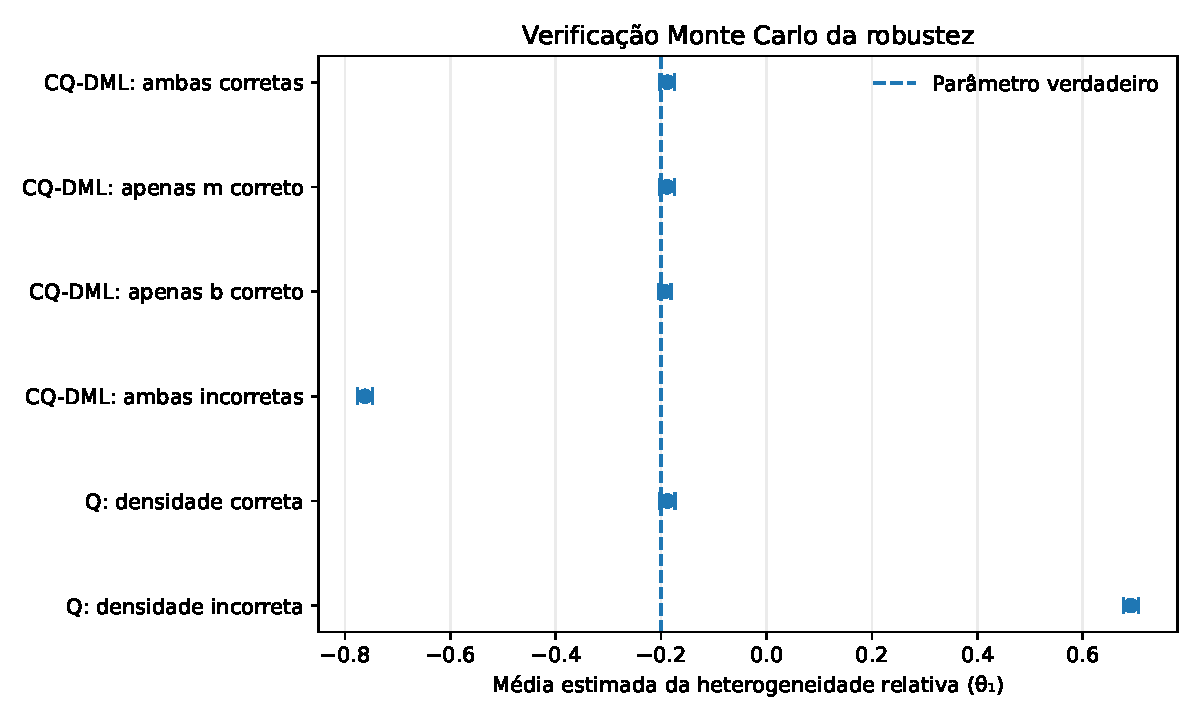
\includegraphics[width=0.97\linewidth]{figures/monte_carlo_robustness.pdf}
\caption{Média do coeficiente de heterogeneidade em 100 replicações. As barras são $1{,}96$ vezes o erro Monte Carlo da média; a linha tracejada é o valor verdadeiro. Dados inteiramente sintéticos.}
\label{fig:mc}
\end{figure}

\subsection{Uma execução com nuisances aprendidas}
Uma realização adicional, com semente 20260906, utilizou $n=100\,000$ e três folds. Um regressor de gradient boosting estimou $\E[T\mid X]$. Um classificador de gradient boosting estimou $\mu(t,x)$, avaliado em $t=0$ para produzir $\hat b$. A função de efeito manteve apenas os dois coeficientes especificados em \eqref{eq:simmu}.

Obtivemos
\[
\hat\theta_0=-0{,}3422\quad (\mathrm{EP}=0{,}0352),\qquad
\hat\theta_1=-0{,}1938\quad (\mathrm{EP}=0{,}0352).
\]
Os intervalos Wald de 95\% foram $[-0{,}4112,-0{,}2731]$ e $[-0{,}2629,-0{,}1248]$. A conversão observada nessa realização foi 6,137\%. Os RMSEs das nuisances em relação à verdade sintética foram 0,0101 para $b$ e 0,0177 para $\E[T\mid X]$. A norma do momento final foi inferior a $4\times10^{-18}$ e o número de condição do Jacobiano foi 7,61.

Essa execução verifica a implementação com previsões fora da amostra; um único conjunto de dados não demonstra cobertura, superioridade ou robustez a mudanças de população.

\subsection{Verificações determinísticas adicionais}
O suplemento computacional confirma por quadratura a identidade \eqref{eq:B} em duas janelas fixas de dose, para todas as combinações de $f$ e $\mu$ corretas/incorretas. As igualdades foram verificadas com tolerância $10^{-10}$. Esses testes validam o resto algébrico, mas não constituem uma avaliação Monte Carlo completa do aprendiz não paramétrico de $\gamma_\pi(x)$.

A Figura~\ref{fig:baseline} mostra uma identidade ilustrativa diferente do DGP Monte Carlo: elasticidade constante de $-2$, com conversões-base de 2\%, 6\% e 25\%. A forma relativa é a mesma, mas os efeitos absolutos diferem. O gráfico não usa dados reais nem estimativas do funil do usuário.
\begin{figure}[htbp]
\centering
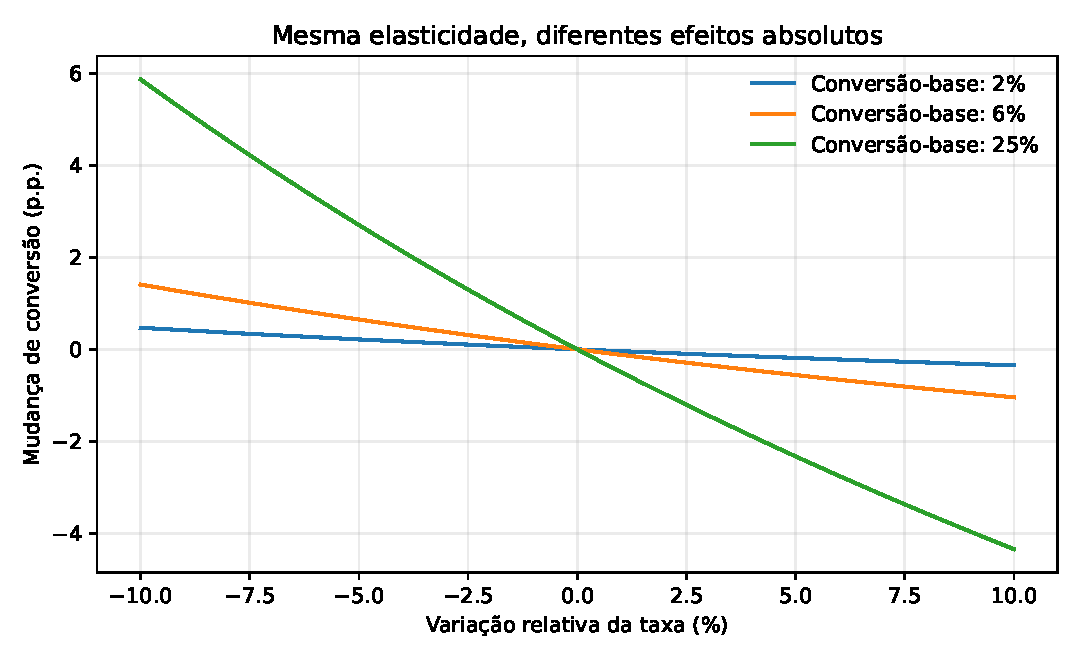
\includegraphics[width=0.88\linewidth]{figures/absolute_vs_relative.pdf}
\caption{Sob elasticidade constante $-2$, a razão de conversões para uma variação relativa $\delta$ da taxa é $(1+\delta)^{-2}$. Multiplicar o lift pelo baseline produz diferentes mudanças em pontos percentuais.}
\label{fig:baseline}
\end{figure}

\section{Pacote Python e dez cenários adicionais}
\label{sec:package}
\subsection{Implementação pragmática e estimandos}
O pacote instalável \texttt{relative-dml}, versão 0.1.0, contém quatro classes. A interface comum usa \texttt{fit}, \texttt{predict\_ratio} e \texttt{predict\_lift}. Fixamos a convenção $\operatorname{lift}=R-1$; por exemplo, $R=1{,}2$ corresponde a lift de 20\%, não a 20 pontos percentuais. As covariáveis devem ser numéricas, finitas e anteriores ao tratamento. A primeira versão considera observações i.i.d.; não implementa inferência por clusters nem uma rotina de otimização comercial.

\texttt{DiscreteQLearner} aplica a identidade multiclasses de \cite{fuchs2026}, ajustando probabilidades de braço na população completa e entre conversores. \texttt{DiscreteDML} estima médias aumentadas por braço. Para $e_j(x)=\Pp(T=j\mid X=x)$, constrói fora do fold
\[
Z_j=\hat\mu_j(X)+\frac{\ind(T=j)}{\hat e_j(X)}\{Y-\hat\mu_j(X)\}.
\]
O resto exato é
\[
\E[Z_j\mid X]-\mu_j(X)
=\left(1-\frac{e_j(X)}{\hat e_j(X)}\right)\{\hat\mu_j(X)-\mu_j(X)\}.
\]
Cada sinal é regressado em $X$; só então formamos a razão das duas médias estimadas. A consistência da razão depende também da consistência das regressões finais e da positividade do denominador. Não dividimos sinais individuais nem cortamos seus valores negativos. Essa opção implementa a alternativa simples discutida após \eqref{eq:relloss}, sem atribuir dupla robustez exata à correção de Taylor do Apêndice~\ref{app:ratio}.

\texttt{ContinuousDML} encapsula o momento já utilizado em \texttt{experiments.py}, com três folds estratificados pelo outcome. A nuisance de baseline é uma classificação de $Y$ em $(X,T)$ avaliada na dose de referência; a média da dose é uma regressão de $T$ em $X$. A base implementada é $(t-t_{\rm ref})[1,V(x)]$, com modificadores $V$ pré-especificados e derivados de $X$. Sem modificadores, há apenas uma inclinação comum. A API não implementa as bases de splines nem o aprendiz de políticas estocásticas discutidos na teoria. Os erros-padrão dos coeficientes mantêm as condições de inferência da Seção~\ref{sec:dml}.

\subsection{Q contínuo por classificação de origens conjuntas}
\texttt{ContinuousQLearner} implementa uma variante simples da classificação de razões de densidade. Construímos uma origem $S=1$ com $(X,T)$ dos conversores e uma origem $S=0$ com $(X,T)$ da população completa. As origens recebem o mesmo peso total. Se $D(x,t)=\Pp(S=1\mid X=x,T=t)$ nessa mistura, então
\[
\frac{D(x,t)}{1-D(x,t)}
=\frac{f_{X,T\mid Y=1}(x,t)}{f_{X,T}(x,t)}
=\frac{\mu(t,x)}{\Pp(Y=1)}.
\]
Portanto, $\logit D(x,t)-\logit D(x,t_0)=\log R(t,t_0;x)$. A referência conjunta mantém a distribuição de alocação observada; a comparação de doses mantém $X$ fixo. Não é necessário simular doses de uma densidade condicional ajustada. O classificador recebe os registros positivos com peso $(n+n_1)/(2n_1)$ e todos os registros com peso $(n+n_1)/(2n)$, onde $n_1=\sum_iY_i$.

Conversores aparecem nas duas origens e não se tornam observações independentes adicionais. Uma eventual validação para tuning deve dividir os registros originais antes dessa duplicação. Esta é uma construção plug-in próxima de um S-learner: não há garantia DR nem alegação de vantagem estatística sobre regressão direta de outcome. Ela difere do Q de inclinação exponencial com densidade pré-fixada do primeiro Monte Carlo. Nas tabelas seguintes, ``Q'' designa a implementação discreta ou contínua correspondente ao cenário.

\subsection{Desenhos, protocolo e escolha do estágio final}
Mantemos $X_1\in\{-1,+1\}$ e $X_2\sim\operatorname{Unif}[-1,1]$, independentes. Nos novos desenhos,
\begin{equation}
\mu(t,x)=B\exp(0{,}65x_1+0{,}4x_2)
\exp\{t(\beta_0+\beta_1x_1)+\kappa t^2\}.
\label{eq:package-dgp}
\end{equation}
O padrão é $B=0{,}04$, $(\beta_0,\beta_1)=(-0{,}35,-0{,}20)$ e $\kappa=0$. No caso contínuo, usamos a densidade de \eqref{eq:simf}, agora com $\alpha(x)=c(0{,}9x_1+0{,}6x_2)$ e $c=1$. No discreto, $\Pp(T=j\mid X=x)=\exp\{j\alpha(x)\}/\sum_{\ell=0}^{K-1}\exp\{\ell\alpha(x)\}$, com braços $j=0,\ldots,K-1$.

Os seis casos contínuos são: efeito nulo ($\beta_0=\beta_1=0$); efeito comum ($\beta_1=0$); heterogêneo (padrão); conversão rara ($B=0{,}008$); pouco overlap ($c=4$); e curva omitida ($\kappa=0{,}8$). Os quatro discretos são: binário aleatorizado ($K=2,c=0$); binário confundido ($K=2,c=1$); três braços ($K=3,c=1$); e binário raro ($K=2,c=1,B=0{,}008$). As probabilidades de \eqref{eq:package-dgp} permanecem em $(0,1)$ nos suportes utilizados; o código também verifica essa condição em cada amostra. A conversão marginal varia por cenário, e não foi fixada em 6\%.

Comparamos Q, DML e um S-learner de conversão em $(X,T)$. As classificações e regressões de nuisance usam histogram gradient boosting com 100 iterações, taxa de aprendizagem 0,1, até oito folhas, pelo menos 50 registros por folha e regularização $L_2=2$. Desativamos early stopping para manter o protocolo explícito. No DML contínuo, $V(x)=x_1$ em todos os casos, inclusive nos efeitos nulo e comum; o ajuste não recebe antecipadamente a informação de que a heterogeneidade é zero. A forma relativa linear favorece esse estimador quando é correta, enquanto Q e S usam classes flexíveis: esta comparação não isola exclusivamente o benefício da ortogonalidade.

Uma rodada piloto de 30 replicações por cenário, semente 20260906, revelou instabilidade na regressão final discreta quando utilizava os mesmos parâmetros das nuisances: houve clipping em todas as 30 replicações de cada caso discreto. Os resultados completos dessa rodada foram preservados em \texttt{results/pilot}. Em resposta, fixamos apenas para o estágio final do DML discreto 30 iterações, taxa de aprendizagem 0,05, até quatro folhas, mínimo de 200 registros por folha e $L_2=10$. Isso regulariza sinais AIPW ruidosos sem substituir o estimando ou truncar os sinais individuais. Os demais modelos ficaram fixos.

A avaliação principal abaixo usa novas sementes, com base 20270906. Para cada cenário e replicação, geramos $n=12\,000$ registros de treino e outros $n_{\rm test}=2\,000$ independentes para avaliação; são 30 replicações por cenário e 900 ajustes, além dos 900 ajustes do piloto. A API de DML usa três folds. No contínuo, avaliamos $t\in\{-0{,}8,-0{,}4,0{,}4,0{,}8\}$ contra zero; no discreto, cada braço não controle contra o braço zero. A verdade é calculada diretamente por \eqref{eq:package-dgp}. Novas sementes separam a avaliação dos dados usados para alterar o estágio final, mas os dez desenhos continuam sendo os mesmos; não se trata de seleção cega de desenhos ou benchmark exaustivo.

\subsection{Métricas e resultados executados}
A métrica principal por replicação é
\[
\operatorname{RMSE}_{\log R}
=\left\{\frac{1}{n_{\rm test}|\mathcal C|}
\sum_{i=1}^{n_{\rm test}}\sum_{t\in\mathcal C}
\big[\log\widehat R(t,0;X_i)-\log R(t,0;X_i)\big]^2\right\}^{1/2}.
\]
Reportamos a média dessa métrica entre replicações; seu erro Monte Carlo é o desvio-padrão das 30 métricas dividido por $\sqrt{30}$. A segunda métrica é o erro absoluto médio do lift, $\E_{\rm teste}|\widehat R-R|$, também calculado por replicação. Um erro de 0,1 corresponde a dez pontos percentuais \emph{na escala do lift relativo}, não na probabilidade de conversão. Os arquivos brutos incluem ainda viés médio do lift, correlação de Spearman na maior dose comparada, contagem de conversores e mensagens de falha e clipping. Spearman fica indefinida para efeito verdadeiro constante.

\begin{table}[htbp]
\centering
\caption{Avaliação principal: média do RMSE de log-ratio e erro Monte Carlo entre parênteses. Trinta replicações, $n=12\,000$ e $n_{\rm test}=2\,000$ por cenário.}
\label{tab:scenarios-log}
\footnotesize
\setlength{\tabcolsep}{4pt}
\begin{tabular}{lrrrr}
\toprule
Cenário & Conv. (\%) & Q & DML & S-learner \\
\midrule
Contínuo: efeito nulo & 4.93 & 0.472 (0.017) & 0.067 (0.006) & 0.370 (0.014) \\
Contínuo: efeito comum & 4.79 & 0.431 (0.026) & 0.076 (0.010) & 0.356 (0.016) \\
Contínuo: heterogêneo & 4.61 & 0.460 (0.020) & 0.079 (0.010) & 0.377 (0.016) \\
Contínuo: conversão rara & 0.94 & 1.064 (0.057) & 0.185 (0.021) & 0.680 (0.038) \\
Contínuo: pouco overlap & 3.88 & 0.564 (0.029) & 0.126 (0.012) & 0.387 (0.018) \\
Contínuo: curva omitida & 6.29 & 0.413 (0.015) & 0.395 (0.003) & 0.333 (0.012) \\
Binário: aleatorizado & 4.07 & 0.462 (0.010) & 0.220 (0.008) & 0.276 (0.010) \\
Binário: confundido & 3.82 & 0.479 (0.012) & 0.273 (0.011) & 0.290 (0.011) \\
Discreto: três braços & 2.84 & 0.699 (0.019) & 0.545 (0.026) & 0.358 (0.009) \\
Binário: conversão rara & 0.72 & 0.896 (0.019) & 0.653 (0.029) & 0.514 (0.027) \\
\bottomrule
\end{tabular}

\end{table}

\begin{table}[htbp]
\centering
\caption{Erro absoluto médio do lift relativo; erro Monte Carlo entre parênteses. Mesmo protocolo da Tabela~\ref{tab:scenarios-log}.}
\label{tab:scenarios-lift}
\footnotesize
\setlength{\tabcolsep}{4pt}
\begin{tabular}{lrrrr}
\toprule
Cenário & Conv. (\%) & Q & DML & S-learner \\
\midrule
Contínuo: efeito nulo & 4.93 & 0.349 (0.022) & 0.055 (0.005) & 0.290 (0.014) \\
Contínuo: efeito comum & 4.79 & 0.323 (0.020) & 0.066 (0.009) & 0.292 (0.013) \\
Contínuo: heterogêneo & 4.61 & 0.369 (0.033) & 0.068 (0.008) & 0.319 (0.022) \\
Contínuo: conversão rara & 0.94 & 1.107 (0.234) & 0.161 (0.018) & 0.619 (0.069) \\
Contínuo: pouco overlap & 3.88 & 0.484 (0.038) & 0.114 (0.011) & 0.313 (0.016) \\
Contínuo: curva omitida & 6.29 & 0.515 (0.036) & 0.430 (0.002) & 0.394 (0.016) \\
Binário: aleatorizado & 4.07 & 0.285 (0.010) & 0.123 (0.006) & 0.153 (0.008) \\
Binário: confundido & 3.82 & 0.311 (0.014) & 0.161 (0.008) & 0.171 (0.010) \\
Discreto: três braços & 2.84 & 0.402 (0.019) & 0.316 (0.042) & 0.173 (0.005) \\
Binário: conversão rara & 0.72 & 1.036 (0.062) & 0.411 (0.024) & 0.326 (0.029) \\
\bottomrule
\end{tabular}

\end{table}

No caso contínuo heterogêneo, o RMSE médio de log-ratio foi 0.079 para DML, 0.460 para Q e 0.377 para S-learner. O DML utiliza aqui a forma relativa correta e apenas dois coeficientes. Seu RMSE aumenta para 0.185 com conversão rara e 0.126 com pouco overlap. Quando se omite curvatura verdadeira, o RMSE do DML chega a 0.395, enquanto o S-learner obtém 0.333. A restrição multiplicativa ajuda nos desenhos que a satisfazem e se torna uma fonte de erro no desenho curvo.

No binário aleatorizado, o DML com estágio final regularizado apresenta RMSE 0.220, frente a 0.462 do Q e 0.276 do S-learner. Essa regularização não resolve todos os regimes: com três braços, os RMSEs de DML e S-learner são 0.545 e 0.358; no binário raro, são 0.653 e 0.514. O S-learner é portanto uma referência relevante, e a garantia de consistência DR não implica menor erro em amostras finitas.

Foram concluídos 900 dos 900 ajustes principais; 0 falhas foram registradas. O DML discreto ainda apresentou clipping em 7/30 replicações com três braços e 8/30 no binário raro. A ausência de avisos no Q não garante precisão: seus erros nos desenhos raros permanecem grandes. As diferenças observadas dependem destes desenhos, classes e parâmetros; não sustentam superioridade geral de uma família.


\begin{figure}[htbp]
\centering
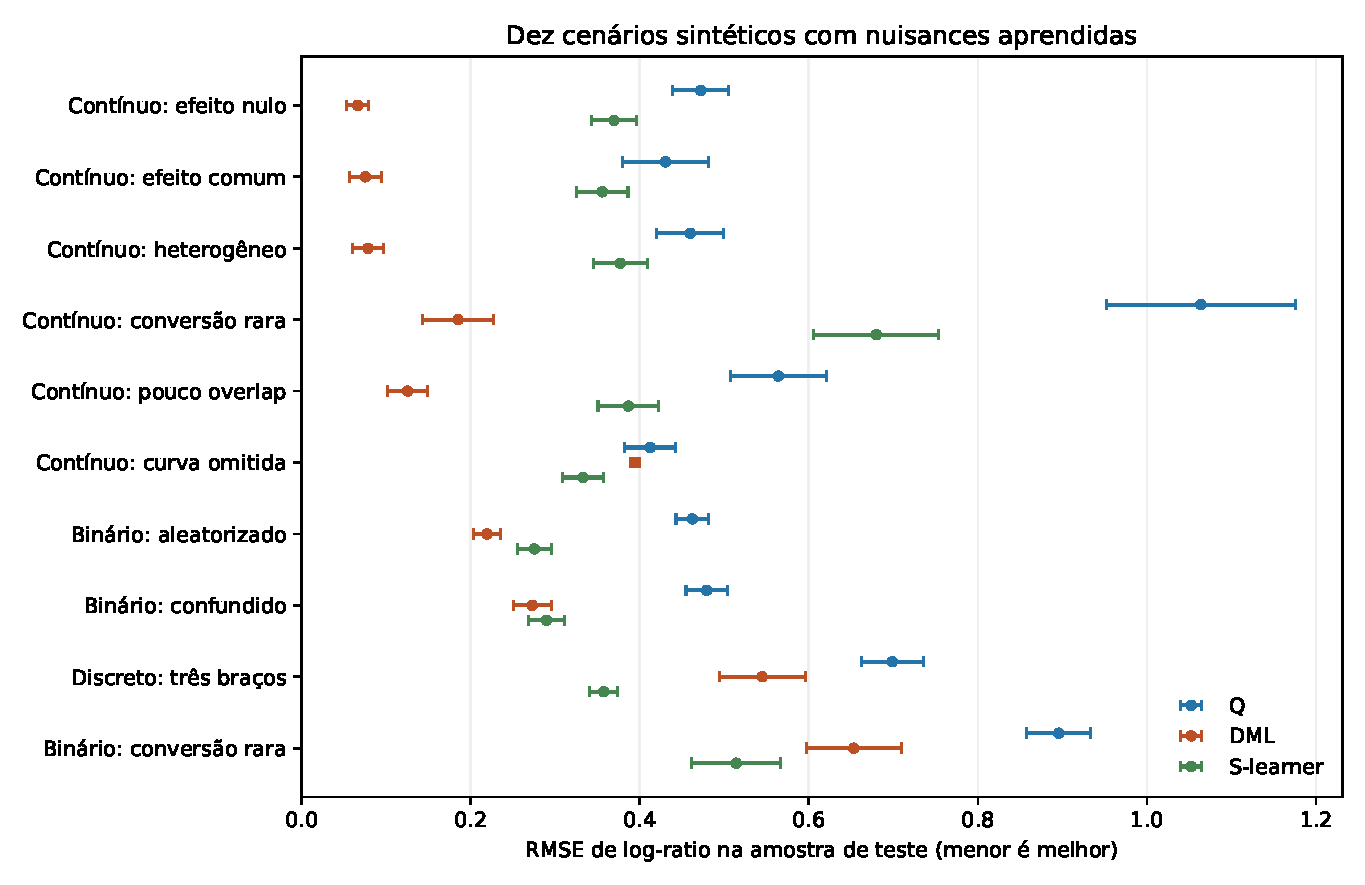
\includegraphics[width=\linewidth]{figures/scenario_comparison.pdf}
\caption{RMSE de log-ratio na amostra independente de teste. As barras são $1{,}96$ vezes o erro Monte Carlo da média das métricas, não intervalos para o efeito de um indivíduo.}
\label{fig:scenarios}
\end{figure}

\subsection{Estabilização, limites e reprodução}
O piso de propensão e de probabilidades usadas nas razões é 0,001. No DML discreto, somente as respostas \emph{após} a regressão final são limitadas a $[0{,}001,1]$; os sinais AIPW podem permanecer negativos. No S-learner, aplicamos o mesmo piso de resposta na avaliação. No Q contínuo, limitamos a probabilidade de origem a $[0{,}001,0{,}999]$; no Q discreto, aplicamos o piso às probabilidades de braço. Esses mecanismos são explicitamente distintos e não tornam iguais as classes de modelos. Um piso fixo pode alterar o alvo efetivo em regiões de baixa conversão ou overlap; resultados com clipping exigem análise de sensibilidade.

\begin{table}[htbp]
\centering
\caption{Replicações com ao menos um aviso de clipping, por cenário e método, na avaliação principal. O numerador conta ajustes, não indivíduos.}
\label{tab:scenarios-clipping}
\small
\begin{tabular}{lrrr}
\toprule
Cenário & Q & DML & S-learner \\
\midrule
Contínuo: efeito nulo & 0/30 & 0/30 & 0/30 \\
Contínuo: efeito comum & 0/30 & 0/30 & 0/30 \\
Contínuo: heterogêneo & 0/30 & 0/30 & 0/30 \\
Contínuo: conversão rara & 0/30 & 0/30 & 20/30 \\
Contínuo: pouco overlap & 0/30 & 0/30 & 0/30 \\
Contínuo: curva omitida & 0/30 & 0/30 & 0/30 \\
Binário: aleatorizado & 0/30 & 0/30 & 0/30 \\
Binário: confundido & 0/30 & 0/30 & 0/30 \\
Discreto: três braços & 0/30 & 7/30 & 0/30 \\
Binário: conversão rara & 0/30 & 8/30 & 21/30 \\
\bottomrule
\end{tabular}

\end{table}

O teste de curvatura é uma falsificação da forma relativa linear, não uma falha das identidades de Bayes ou do resto DR sob seu modelo correto. O caso de pouco overlap ainda tem densidade positiva em todo $[-1,1]$, mas atribui pouca informação a algumas comparações; nenhuma restrição de intervalo global verifica suporte condicional. A conversão rara reduz informação para todos os métodos. As tabelas não demonstram cobertura de intervalos de confiança nem consistência assintótica a partir de uma única dimensão amostral.

\texttt{scenario\_experiments.py} gera os dados e os CSVs; \texttt{make\_scenario\_figures.py} produz automaticamente as duas tabelas de métricas, a tabela de avisos e a figura a partir desses CSVs. Metadados registram versões efetivamente usadas, sementes e parâmetros. A rodada piloto pode ser reproduzida com \texttt{--seed 20260906 --pilot-final}; a avaliação principal usa a semente padrão 20270906. O pacote possui testes de identidades em populações finitas, braço multiclasses, referência não nula, recuperação de heterogeneidade e exclusão dos registros de treino nas predições de nuisance. Esses testes complementam o Monte Carlo, sem substituir validação em dados reais.


\section{Discussão e conclusão}
A perspectiva Q estende-se ao tratamento contínuo e outcome binário por uma identidade exata: a resposta relativa é a alteração da densidade de dose entre conversores, corrigida pela densidade de alocação. Essa identidade explica por que uma forma relativa pode ser aprendida sem confundi-la algebraicamente com o nível de conversão.

Ela não oferece dupla robustez automaticamente. Uma rota regular é especificar a forma log-relativa e usar um momento multiplicativo residualizado, cuja identidade de viés é exatamente bilinear. Uma rota não paramétrica é substituir doses pontuais por intervenções fixas, estimar duas médias com sinais aumentados e aprender sua razão por uma equação de momentos. As duas rotas respondem a perguntas diferentes e têm pressupostos diferentes.

Para precificação de financiamento, a recomendação metodológica é manter separados o nível de conversão, a forma relativa da resposta e o valor econômico por contrato. Começar com uma curva relativa comum fornece um benchmark substantivo. Heterogeneidade adicional só é útil quando reproduzida em doses comparáveis e fora da amostra. A ausência de ordenação clara dos lifts pode refletir homogeneidade relativa ou falta de informação; não pode ser decidida pelo score aditivo isoladamente.

O manuscrito não estabelece que um novo estimador domine os existentes, não resolve confundimento não observado e não demonstra novidade editorial suficiente para publicação. Os dez desenhos adicionais tornam explícitos os efeitos de curvatura, overlap, prevalência e regularização na implementação inicial. O próximo avanço científico exigiria comparação com G-estimação eficiente, modelos multiplicativos compatíveis, estimadores contínuos DR e outros aprendizes de razões, ampliando tamanhos amostrais, formas de heterogeneidade e validação em dados reais. A contribuição entregue é uma construção teórica verificável, com pacote Python e evidência sintética delimitada.

\appendix
\section{Por que uma correção de primeira ordem de uma razão pode não ser DR}
\label{app:ratio}
Considere $u_0/v_0$ e estimativas iniciais $\hat u,\hat v$. Mesmo que haja sinais de correção com esperanças $u_0-\hat u$ e $v_0-\hat v$, a correção de primeira ordem
\[
\widehat R+\frac{u_0-\hat u}{\hat v}
-\widehat R\frac{v_0-\hat v}{\hat v},\qquad
\widehat R=\frac{\hat u}{\hat v},
\]
tem diferença em relação a $R_0=u_0/v_0$ igual a
\[
\left(1-\frac{v_0}{\hat v}\right)(\widehat R-R_0).
\]
Esse resto é de segunda ordem perto da verdade, mas não precisa desaparecer sob misspecificação persistente. Assim, ortogonalidade local não basta para provar dupla robustez de consistência. As equações \eqref{eq:product} e \eqref{eq:B} evitam essa ambiguidade ao exibir o resto exato nos blocos de nuisance relevantes.

Por exemplo, com $(u_0,v_0)=(0{,}2,0{,}1)$ e $(\hat u,\hat v)=(0{,}3,0{,}2)$, o ratio verdadeiro é 2, mas a correção acima vale $1{,}5-0{,}5+0{,}75=1{,}75$, mesmo quando a propensão correta fornece as esperanças exatas dos resíduos. Esse contraexemplo numérico também integra os testes do pacote; ele distingue explicitamente o resto de Taylor de dupla robustez exata.

\section{A restrição log-linear sob misspecificação}
\label{app:misspec}
Se a verdadeira resposta é $\mu(t,x)=b_0(x)e^{g_0(t,x)}$, mas o estimador usa $g_\theta=\theta^{\mathsf T}H$, o momento com $m=m_0$ passa a ter esperança
\[
\E\left[(H-m_0)b_0(X)e^{g_0(T,X)-g_\theta(T,X)}\right].
\]
O termo envolvendo a nuisance $b$ ainda cancela pela centralização, mas a raiz depende de toda a distribuição de $(T,X)$ e da discrepância de forma. Não há uma razão para igualá-la à derivada local de $g_0$ em uma dose específica. Esse é o motivo para validar curvatura ou usar o alvo estocástico não paramétrico.

\section{Detalhes da densidade sintética e da reprodução}
A função $M(z)=\sinh(z)/z$ é a função geradora de momentos de uma uniforme em $[-1,1]$. A média sob inclinação $z$ é
\[
\E[T\mid z]=\frac{d}{dz}\log M(z)=\coth z-\frac1z,
\]
com extensão contínua zero em $z=0$. A variância é $1/z^2-1/\sinh^2z$, com limite $1/3$. O código usa expansões em série perto de zero para estabilidade numérica.

A calibração da conversão esperada utiliza
\[
\E[Y]=c\,\E_X\left[\exp(1{,}1X_1+0{,}7X_2)
\frac{M\{\alpha(X)+\theta_0+\theta_1X_1\}}{M\{\alpha(X)\}}\right].
\]
Os resultados originais podem ser reproduzidos executando \texttt{experiments.py}; os dez cenários adicionais usam \texttt{scenario\_experiments.py}. O diretório \texttt{results} contém saídas brutas, resumos Monte Carlo, metadados, verificações de quadratura e a execução de ML. O arquivo \texttt{README.md} descreve o ambiente, comandos e limites. A rotina central \texttt{fit\_multiplicative\_dml}, agora importada do pacote, exige nuisances fora da amostra ou pré-fixadas; passar predições treinadas nos próprios outcomes viola o protocolo de cross-fitting utilizado na análise.

\clearpage
\section{Guia prático: o que aparece nos quantis de cada score?}
\label{app:quantiles}

\subsection{Antes de ordenar: duas perguntas diferentes}
Imagine uma ação que pode aumentar a conversão. Para cada perfil de cliente, conhecemos a probabilidade de converter sem a ação, $\mu_0(x)=\mu(a_0,x)$, e com a ação, $\mu_1(x)=\mu(a,x)$. Aqui, ``com ação'' significa aplicar a mesma alternativa $a$ a todos; ``sem ação'' significa aplicar a mesma referência $a_0$. Os exemplos são inteiramente fictícios, com probabilidades conhecidas. Não há modelos ajustados, outcomes sorteados ou erro de estimação.

Dois scores respondem a perguntas úteis, mas diferentes:
\begin{align*}
S_{\mathrm{CATE}}(x)&=\mu_1(x)-\mu_0(x)
&&\text{(quanto aumenta a chance de converter?)},\\
S_{\mathrm{lift}}(x)&=\frac{\mu_1(x)}{\mu_0(x)}-1
&&\text{(quanto aumenta em relação à chance inicial?)}.
\end{align*}
\textbf{CATE é um ganho absoluto; lift é um ganho proporcional.} Neste apêndice, CATE sempre designa a diferença aditiva. O score relativo também pode ser expresso como razão $R=1+\mathrm{lift}$ ou log-razão $g=\log(1+\mathrm{lift})$: ambos produzem o mesmo ranking do lift, pois são transformações estritamente crescentes.

\noindent\textbf{Unidades, sem ambiguidade.} Passar de 2\% para 3,6\% significa ganhar \emph{1,6 ponto percentual}, ou 0,016 na escala de probabilidade. O lift é $3{,}6/2-1=80\%$. Em 1\,000 pessoas iguais a esse perfil, isso corresponde a passar de 20 para 36 conversões esperadas: \emph{16 conversões adicionais}. São expectativas contrafactuais, não a identificação de quais 16 pessoas mudariam de decisão.

\begin{table}[H]
\centering\small
\caption{Cinco perfis fictícios, cada um com 20\% da população. O contraste de tratamento é o mesmo em todas as linhas.}
\label{tab:quantile_profiles}
\begin{tabular}{lrrrrr}
\toprule
Perfil & Pessoas & Base (\%) & Com ação (\%) & CATE (p.p.) & Lift (\%) \\
\midrule
A & 1000 & 2,00 & 3,60 & 1,60 & 80,00 \\
B & 1000 & 4,00 & 6,00 & 2,00 & 50,00 \\
C & 1000 & 8,00 & 10,40 & 2,40 & 30,00 \\
D & 1000 & 16,00 & 19,20 & 3,20 & 20,00 \\
E & 1000 & 25,00 & 28,75 & 3,75 & 15,00 \\
\bottomrule
\end{tabular}

\end{table}

\textbf{A e E deixam a diferença clara.} O perfil A ganha 80\% sobre uma base de 2\%: seu CATE é 1,6 p.p. O perfil E ganha 15\% sobre uma base de 25\%: seu CATE é 3,75 p.p. Portanto, A tem o maior lift e E tem o maior ganho absoluto. Isso decorre da identidade
\[
\underbrace{\mathrm{CATE}(x)}_{\text{ganho absoluto}}
=\underbrace{\mu_0(x)}_{\text{conversão-base}}
\times\underbrace{\mathrm{lift}(x)}_{\text{ganho relativo}}.
\]
Um método DML pode aprender um alvo aditivo ou relativo, dependendo da equação usada. ``DML'' descreve a construção de estimação e não determina a unidade do score. No pacote deste projeto, os Q-Learners e os DMLs entregam respostas relativas; o CATE aditivo exige também uma estimativa de $\mu_0(x)$, multiplicada pelo lift.

\clearpage
\subsection{Os mesmos clientes, duas ordenações e cinco grupos}
Ordenamos as 5\,000 pessoas do menor para o maior score e formamos cinco grupos de 1\,000: \textbf{Q1 tem os menores scores e Q5 os maiores}. Cada perfil tem um score distinto e ocupa exatamente um quintil; nenhum empate é dividido. Na tabela, ``extras'' significa $1\,000\times\mathrm{CATE}$, e lift do grupo significa razão das suas médias de conversão, menos um.

\begin{table}[H]
\centering\small
\setlength{\tabcolsep}{5pt}
\caption{O que se encontra em cada quintil. A população é a mesma; apenas a ordenação muda.}
\label{tab:quantile_rankings}
\begin{tabular}{lllrrrrr}
\toprule
Score & Quantil & Perfil & \shortstack{Base\\(\%)} & \shortstack{Com ação\\(\%)} & \shortstack{CATE\\(p.p.)} & \shortstack{Lift\\(\%)} & \shortstack{Extras por\\1\,000} \\
\midrule
CATE & Q1 & A & 2,00 & 3,60 & 1,60 & 80,00 & 16,0 \\
CATE & Q2 & B & 4,00 & 6,00 & 2,00 & 50,00 & 20,0 \\
CATE & Q3 & C & 8,00 & 10,40 & 2,40 & 30,00 & 24,0 \\
CATE & Q4 & D & 16,00 & 19,20 & 3,20 & 20,00 & 32,0 \\
CATE & Q5 & E & 25,00 & 28,75 & 3,75 & 15,00 & 37,5 \\
Lift & Q1 & E & 25,00 & 28,75 & 3,75 & 15,00 & 37,5 \\
Lift & Q2 & D & 16,00 & 19,20 & 3,20 & 20,00 & 32,0 \\
Lift & Q3 & C & 8,00 & 10,40 & 2,40 & 30,00 & 24,0 \\
Lift & Q4 & B & 4,00 & 6,00 & 2,00 & 50,00 & 20,0 \\
Lift & Q5 & A & 2,00 & 3,60 & 1,60 & 80,00 & 16,0 \\
\bottomrule
\end{tabular}

\end{table}

\begin{figure}[H]
\centering
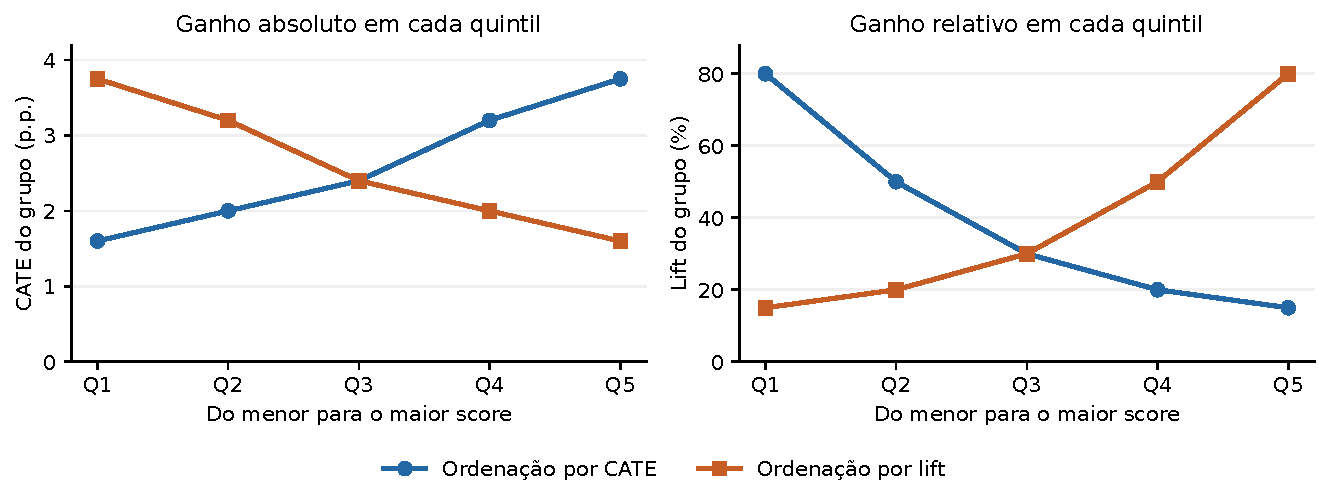
\includegraphics[width=\linewidth]{figures/quantile_cate_vs_lift.pdf}
\caption{Azul: grupos formados pelo score de CATE. Laranja: grupos formados pelo score de lift. Cada painel avalia ambos os rankings na mesma unidade. Q5 reúne pessoas diferentes nas duas curvas. Valores exatos da população sintética, sem incerteza amostral.}
\label{fig:quantile_rankings}
\end{figure}

\textbf{Como ler o gráfico.} O ranking azul cresce no painel de CATE, mas cai no de lift. O laranja faz o inverso. Um score pode ordenar perfeitamente o seu alvo e ter uma curva decrescente na outra escala. Isso não é falha de calibração: os alvos são diferentes.

\textbf{Se só houver capacidade para 1\,000 pessoas:} selecionar Q5 por CATE escolhe E e gera 37,5 conversões adicionais esperadas; selecionar Q5 por lift escolhe A e gera 16. Com custo e valor por conversão iguais, o primeiro maximiza conversões incrementais neste exemplo. O segundo seleciona a maior resposta proporcional. Lift alto, isoladamente, não significa maior lucro ou maior número de conversões extras.

\clearpage
\subsection{Quando o lift empata: o baseline pode ordenar o CATE}
Agora mantenha as mesmas conversões-base e imponha um lift de 20\% para todos. A conversão aumenta proporcionalmente da mesma forma em todos os perfis, enquanto o ganho em pontos percentuais aumenta com o baseline.

\begin{table}[H]
\centering\small
\caption{Resposta relativa constante: todos têm o mesmo lift.}
\label{tab:quantile_constant}
\begin{tabular}{lrrrr}
\toprule
Perfil & Base (\%) & Com ação (\%) & CATE (p.p.) & Lift (\%) \\
\midrule
A & 2,00 & 2,40 & 0,40 & 20,00 \\
B & 4,00 & 4,80 & 0,80 & 20,00 \\
C & 8,00 & 9,60 & 1,60 & 20,00 \\
D & 16,00 & 19,20 & 3,20 & 20,00 \\
E & 25,00 & 30,00 & 5,00 & 20,00 \\
\bottomrule
\end{tabular}

\end{table}

O score de CATE ordena A, B, C, D e E; seus quintis coincidem com a ordem do baseline. O score de lift vale 20\% para todas as pessoas: \textbf{não existem cinco faixas distintas de resposta relativa}. Um software pode desempatar por posição da linha ou aleatoriamente, mas esses grupos não representam diferenças de lift. Por isso, não fabricamos uma curva de quintis relativos neste caso. Se um modelo estimado produzir pequenas diferenças, a ordenação pode refletir apenas ruído e precisa de validação fora da amostra.

\subsection{A média dos lifts individuais pode não ser o lift do grupo}
Para um grupo $G$, as quantidades usadas na tabela e no gráfico são
\[
\mathrm{CATE}_G=\E[\mu_1(X)\mid G]-\E[\mu_0(X)\mid G],\qquad
\mathrm{lift}_G=\frac{\E[\mu_1(X)\mid G]}{\E[\mu_0(X)\mid G]}-1.
\]
A média dos CATEs individuais é o CATE do grupo. A média simples dos lifts individuais, em geral, não é o lift do grupo. Veja dois perfis de mesmo tamanho:

\begin{table}[H]
\centering\small
\caption{Dois perfis com pesos iguais: média individual de 55\%, lift do grupo de 18,18\%.}
\label{tab:quantile_mixture}
\begin{tabular}{lrrrr}
\toprule
Perfil & Base (\%) & Com ação (\%) & CATE (p.p.) & Lift (\%) \\
\midrule
U & 1,00 & 2,00 & 1,00 & 100,00 \\
V & 10,00 & 11,00 & 1,00 & 10,00 \\
Grupo (médias) & 5,50 & 6,50 & 1,00 & 18,18 \\
\bottomrule
\end{tabular}

\end{table}

A média dos lifts é $(100\%+10\%)/2=55\%$. Porém, a conversão média passa de 5,5\% para 6,5\%, de modo que o lift do grupo é $6{,}5/5{,}5-1=18{,}18\%$. A fórmula correta é
\[
\mathrm{lift}_G
=\frac{\E[\mu_0(X)\,\mathrm{lift}(X)\mid G]}{\E[\mu_0(X)\mid G]}:
\]
os pesos são proporcionais às conversões-base esperadas. A média simples de 55\% é outro resumo legítimo, desde que seja rotulada como \emph{média dos lifts individuais}. No exemplo principal, cada quintil contém um único perfil, então os dois resumos coincidem dentro do quintil. Na população inteira, o CATE é 2,59 p.p. e o lift do grupo é 23,55\%, independentemente do ranking escolhido.

\clearpage
\subsection{O mesmo raciocínio vale para tratamento contínuo}
Em um tratamento discreto, podemos comparar braço 1 com braço 0. Em um tratamento contínuo, precisamos fixar duas doses e a direção da mudança: por exemplo, $a_0=0$ e $a=1$ em uma escala normalizada. Uma curva que reproduz exatamente os cinco perfis da Tabela~\ref{tab:quantile_profiles} é
\[
\mu(t,x)=b(x)\exp\{t\log(1+\ell(x))\},\qquad 0\leq t\leq1,
\]
com $b(x)$ igual ao baseline e $\ell(x)$ igual ao lift daquela tabela. Em $t=0$, a conversão é $b(x)$; em $t=1$, é $b(x)(1+\ell(x))$. Todas as probabilidades permanecem entre zero e um. Para o contraste $0\to1$, os CATEs, lifts e rankings são os mesmos do exemplo discreto.

Para outra mudança $a_0\to a$, o score relativo nessa curva passa a ser
\[
\mathrm{lift}(a,a_0;x)=\exp\{(a-a_0)\log(1+\ell(x))\}-1,
\]
e o score absoluto é $\mu(a_0,x)\times\mathrm{lift}(a,a_0;x)$. \textbf{A comparação precisa usar o mesmo contraste nos dois scores.} Uma derivada $s(t,x)=\partial_t\log\mu(t,x)$ mede variação log-relativa por unidade de dose; ela não é o lift de uma mudança finita. Nesta curva, $s=\log(1+\ell)$, e o lift requer aplicar a exponencial ao produto da inclinação pela mudança de dose. Se a curva tiver curvatura, usa-se a diferença de log-respostas entre as duas doses, ou a integral de $s$, e não apenas uma derivada local.

\subsection{Como fazer a avaliação com scores aprendidos}
Os exemplos anteriores ensinam a ler o alvo, não demonstram a qualidade preditiva de um estimador. Com dados observados, um protocolo simples é:
\begin{enumerate}
\item \textbf{Definir a comparação antes de avaliar.} Fixar população, outcome, janela temporal, doses ou braços e escala do tratamento. Construir um score para CATE e outro para lift para esse mesmo contraste.
\item \textbf{Separar treino de avaliação.} Treinar os modelos em uma amostra e congelar suas previsões antes de usar os outcomes de teste. Formar os quintis a partir dessas previsões, sem consultar os outcomes. Registrar os cortes e o tratamento dos empates; para comparação, usar a mesma população de teste nos dois rankings.
\item \textbf{Estimar as duas conversões em cada grupo.} Em um experimento binário com probabilidades de alocação constantes, médias por braço são uma referência; com alocação variável, usar os pesos do desenho. Em dados observacionais discretos, usar médias ajustadas, por exemplo sinais AIPW com nuisances fora da amostra e overlap adequado. Para dose contínua, usar o estimador de dose-resposta ou de intervenção estocástica apropriado: não basta aplicar a fórmula AIPW binária a doses exatas.
\item \textbf{Mostrar as duas escalas e sua incerteza.} A partir das médias estimadas, calcular diferença em p.p. e razão menos um. Reportar tamanho do grupo, conversão-base, suporte e intervalos compatíveis com o desenho. Uma curva monotônica de previsões por construção não valida o efeito; a evidência vem da avaliação independente dos grupos.
\end{enumerate}
Comparar apenas a conversão observada de Q5 com a de Q1 mistura baseline, composição dos grupos e alocação de tratamento. Isso não identifica CATE nem lift causal. Em dados sintéticos podemos calcular as duas médias contrafactuais exatas; em dados reais é necessário estimá-las sob as hipóteses de identificação.

\noindent\textbf{Reprodução.} Executar \texttt{quantile\_examples.py} recria as tabelas, CSVs e o gráfico. O script verifica as identidades de agregação, a inversão do perfil selecionado em Q5, o empate de lift constante e o contraexemplo da média dos lifts.


\begin{thebibliography}{99}
\small
\setlength{\itemsep}{2pt}
\setlength{\parskip}{0pt}
\bibitem{fuchs2026} Fuchs, M.; Kreiss, D. (2026). \emph{Beyond Differences: Doubly Robust Meta-Learners for Ratio-Based Treatment Effects}. arXiv:2605.26288v1, 25 maio 2026. \url{https://arxiv.org/abs/2605.26288}.
\bibitem{yin2022} Yin, J.; Markes, S.; Richardson, T. S.; Wang, L. (2022). \emph{Multiplicative Effect Modeling: The General Case}. arXiv:1906.00558v4, 3 janeiro 2022. \url{https://arxiv.org/abs/1906.00558}.
\bibitem{dukes2018} Dukes, O.; Vansteelandt, S. (2018). A Note on G-Estimation of Causal Risk Ratios. \emph{American Journal of Epidemiology}, 187(5), 1079--1084. doi:10.1093/aje/kwx347.
\bibitem{yadlowsky2021} Yadlowsky, S.; Pellegrini, F.; Lionetto, F.; Braune, S.; Tian, L. (2021). Estimation and Validation of Ratio-based Conditional Average Treatment Effects Using Observational Data. \emph{Journal of the American Statistical Association}, 116(533), 335--352. \url{https://arxiv.org/abs/1912.06977}.
\bibitem{chernozhukov2018} Chernozhukov, V.; Chetverikov, D.; Demirer, M.; Duflo, E.; Hansen, C.; Newey, W.; Robins, J. (2018). Double/debiased machine learning for treatment and structural parameters. \emph{The Econometrics Journal}, 21(1), C1--C68. doi:10.1111/ectj.12097.
\bibitem{kennedy2017} Kennedy, E. H.; Ma, Z.; McHugh, M. D.; Small, D. S. (2017). Non-parametric methods for doubly robust estimation of continuous treatment effects. \emph{Journal of the Royal Statistical Society, Series B}, 79(4), 1229--1245. doi:10.1111/rssb.12212.
\bibitem{colangelo2020} Colangelo, K.; Lee, Y.-Y. (2020). \emph{Double Debiased Machine Learning Nonparametric Inference with Continuous Treatments}. arXiv:2004.03036. \url{https://arxiv.org/abs/2004.03036}.
\bibitem{diaz2012} Díaz Muñoz, I.; van der Laan, M. J. (2012). Population Intervention Causal Effects Based on Stochastic Interventions. \emph{Biometrics}, 68(2), 541--549. doi:10.1111/j.1541-0420.2011.01685.x.
\bibitem{ge2026} Ge, J.; Díaz, I. (2026). \emph{Orthogonal machine learning for conditional odds and risk ratios}. arXiv:2604.10412v1, 12 abril 2026. \url{https://arxiv.org/abs/2604.10412}.
\bibitem{shinoda2022} Shinoda, K.; Hoshino, T. (2022). \emph{Orthogonal Series Estimation for the Ratio of Conditional Expectation Functions}. arXiv:2212.13145. \url{https://arxiv.org/abs/2212.13145}.
\bibitem{sugiyama2012} Sugiyama, M.; Suzuki, T.; Kanamori, T. (2012). \emph{Density Ratio Estimation in Machine Learning}. Cambridge University Press.
\bibitem{dukes2024} Dukes, O.; Vansteelandt, S.; Whitney, D. (2024). On Doubly Robust Inference for Double Machine Learning in Semiparametric Regression. \emph{Journal of Machine Learning Research}, 25(279), 1--46. \url{https://jmlr.org/papers/v25/22-1233.html}.
\end{thebibliography}
\end{document}
